\documentclass{beamer}

\usepackage{multimedia}
\usepackage{tabularx}

\usepackage{caption}
\usepackage{subcaption}

\usepackage{mathtools}

\usepackage[absolute,overlay]{textpos}

\setbeamercolor{framesource}{fg=gray}
\setbeamerfont{framesource}{size=\tiny}

\newcommand{\source}[1]{\begin{textblock*}{4cm}(0.2cm,8.6cm)
    \begin{beamercolorbox}[ht=0.5cm,left]{framesource}
        \usebeamerfont{framesource}\usebeamercolor[fg]{framesource} Source: {#1}
    \end{beamercolorbox}
\end{textblock*}}

\newcommand{\rulesep}{\unskip\ \vrule\ }

\setbeamercolor{subsection header}{fg=title.fg,bg=title.bg!75}
\setbeamercolor{subsubsection header}{fg=title.fg,bg=title.bg!50}

%tikzpicture
\usepackage{tikz}
\usepackage{scalerel}
\usepackage{pict2e}
\usepackage{tkz-euclide}
\usetikzlibrary{calc}
\usetikzlibrary{patterns,arrows.meta}
\usetikzlibrary{shadows}
\usetikzlibrary{external}

%pgfplots
\usepackage{pgfplots}
\pgfplotsset{compat=newest}
\usepgfplotslibrary{statistics}
\usepgfplotslibrary{fillbetween}

% Preamble:
\usepackage{adjustbox}


\usetheme{Madrid}
\setbeamercovered{transparent}

\title{Game Theory for Image Segmentation}
\subtitle{\textit{Controversies in Game Theory IX}}
\author[Clément JAMBON]{Clément JAMBON}
\institute[]{ETH Zürich}
\titlegraphic{
    \centering
    \begin{columns}
        \begin{column}{0.5\textwidth}
           \centering
           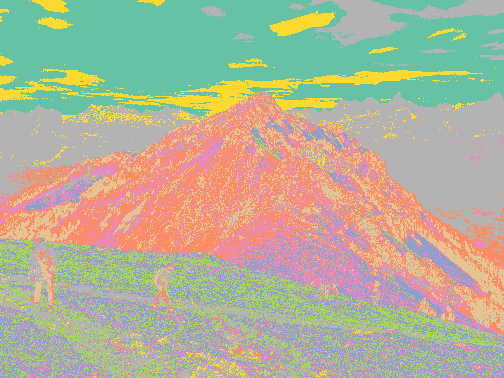
\includegraphics[width=4cm]{../figures/teaser/hike_seg.png}
        \end{column}
        \begin{column}{0.5\textwidth}  %%<--- here
           \centering
           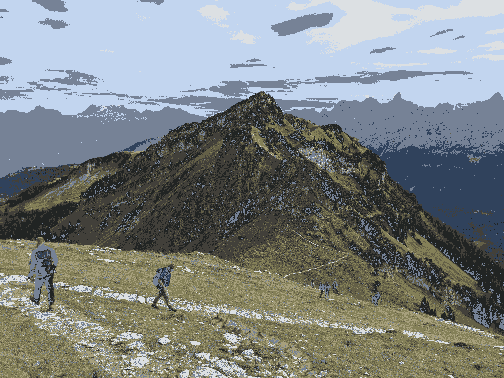
\includegraphics[width=4cm]{../figures/teaser/hike_avg.png}
        \end{column}
    \end{columns}    
}

\begin{document}

\frame{\titlepage}

\begin{frame}
    \frametitle{Overview}

    \begin{itemize}
        \item Image Segmentation has been extensively studied in the Image Processing community for decades.
        \item We propose to build on the PhD dissertation of Samuel Rota Bulò\cite{bulo-thesis} and the publication of Shen et al.~\cite{game-clustering} and reproduce their results.
        \item To do so, we formulate Image Segmentation as a clustering game, which we simulate through discrete-time evolutionary dynamics.
        \item More precisely, we investigate and evaluate three approaches: \textit{Best response dynamics}, \textit{Replicator dynamics} and \textit{Infection and immunization dynamics}\cite{inimdyn}.
        \item Additionally, we extend their results to semantic segmentation by making use of state-of-the-art self-supervised features, namely DINO\cite{dino} features.
    \end{itemize}

\end{frame}

\begin{frame}
    \frametitle{Image Segmentation as a clustering game}
    Image Segmentation can be defined as a clustering game where:
    \begin{itemize}
        \item Pixels $\{1, \ldots, n\}$ are represented as a mixed strategy $(x_1, \ldots, x_n)$ in the simplex $\Delta$ i.e.~ $\sum_{i=1}^nx_i=1$.
        \item The payoff of a pixel $i$ against another pixel $j$ is given by a similarity matrix $A\in\mathbb{R}^{n\times n}$ that quantify how close two pixels are from one another.
        \item In practice, we choose a Gaussian kernel $A_{i, j}=\exp\left(-\frac{\lVert C(i) - C(j)\rVert^2}{\sigma^2}\right)$ where $C(i)$ is a 3-dimensional vector representing the value of pixel $i$.
        \item The goal of the clustering game is to find a Nash equilibrium w.r.t. this setting.
    \end{itemize}
\end{frame}

\begin{frame}
    \frametitle{Evolutionary dynamics}
    In order to solve such a high dimensional problem, we use evolutionary dynamics and three different discrete-time dynamics:
    \begin{enumerate}
        \item \textit{Best response dynamics} which inject in the population, at each time step, one individual that would yield the best response w.r.t. the payoff matrix.
        \item \textit{Replicator dynamics} that can be seen as a form of \textit{Darwin selection} whereby the "fittest" populations are more inclined to survive.
        \item \textit{Infection and immunization dynamics} where "infectious" individuals are iteratively introduced in a population to yield immunity.
    \end{enumerate}
    We refer the reader to our report for more rigorous definition and our Python notebook for a practical implementation of these approaches.
\end{frame}

\begin{frame}
    \frametitle{Results}
    \begin{figure}
        \centering
        \begin{subfigure}[b]{0.25\textwidth}
            \centering
            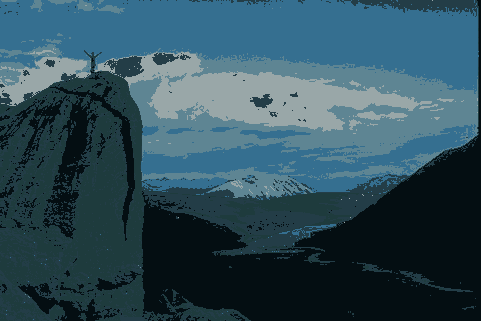
\includegraphics[width=\textwidth]{../figures/methods/fp/14037_avg.png}
            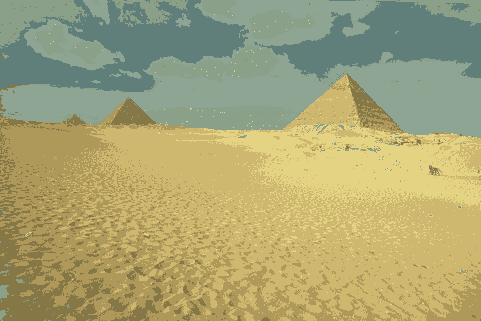
\includegraphics[width=\textwidth]{../figures/methods/fp/260058_avg.png}
            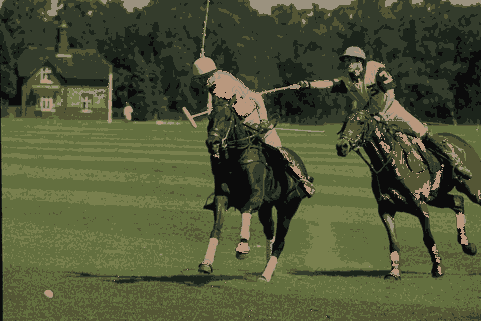
\includegraphics[width=\textwidth]{../figures/methods/fp/361010_avg.png}
            \caption{Best Response dynamics}
        \end{subfigure}
        \hfill
        \begin{subfigure}[b]{0.25\textwidth}
            \centering
            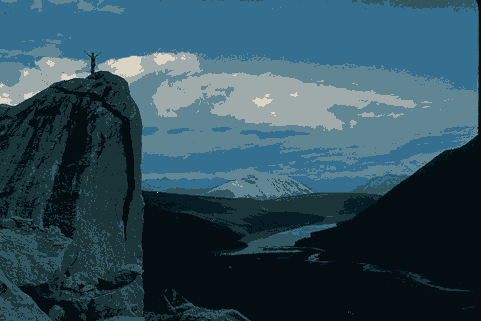
\includegraphics[width=\textwidth]{../figures/methods/rd/14037_avg.png}
            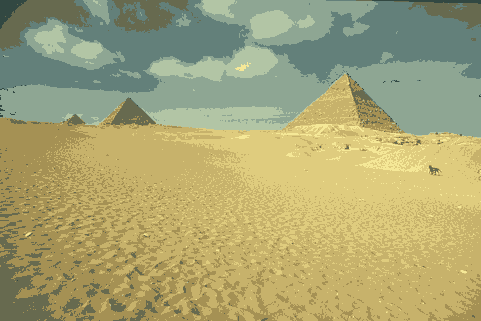
\includegraphics[width=\textwidth]{../figures/methods/rd/260058_avg.png}
            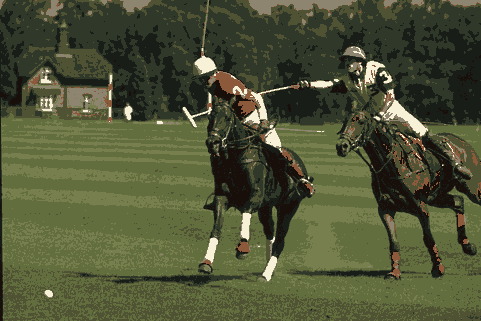
\includegraphics[width=\textwidth]{../figures/methods/rd/361010_avg.png}
            \caption{Replicator dynamics}
        \end{subfigure}
        \hfill
        \begin{subfigure}[b]{0.25\textwidth}
            \centering
            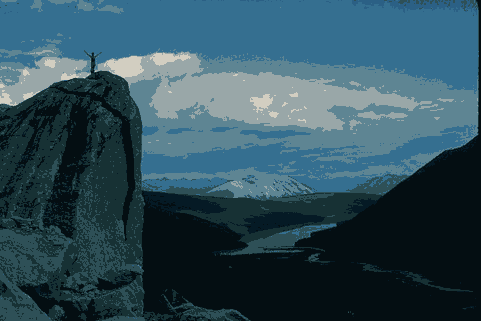
\includegraphics[width=\textwidth]{../figures/methods/inimdyn/14037_avg.png}
            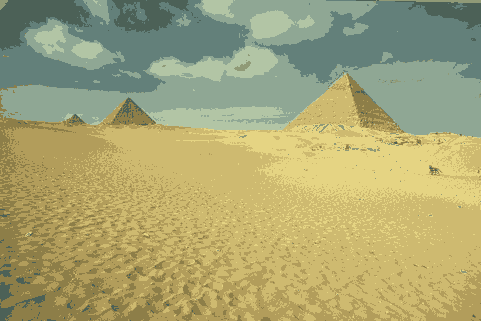
\includegraphics[width=\textwidth]{../figures/methods/inimdyn/260058_avg.png}
            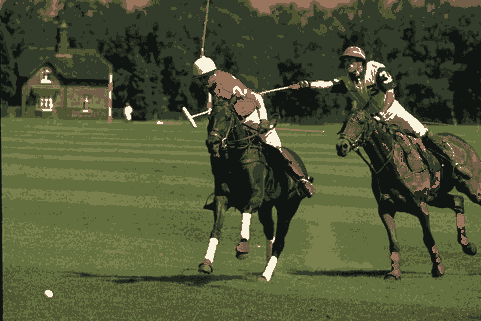
\includegraphics[width=\textwidth]{../figures/methods/inimdyn/361010_avg.png}
            \caption{Pure InImDyn}
        \end{subfigure}
           \caption{Segmentations obtained with our implementations of the three dynamics presented in section \ref{sec:evo-dyn} at sampling rate $p=0.01$.}
           \label{fig:results-dynamics}
    \end{figure}
\end{frame}

\begin{frame}
    \frametitle{Results}
    \begin{figure}
        \centering
        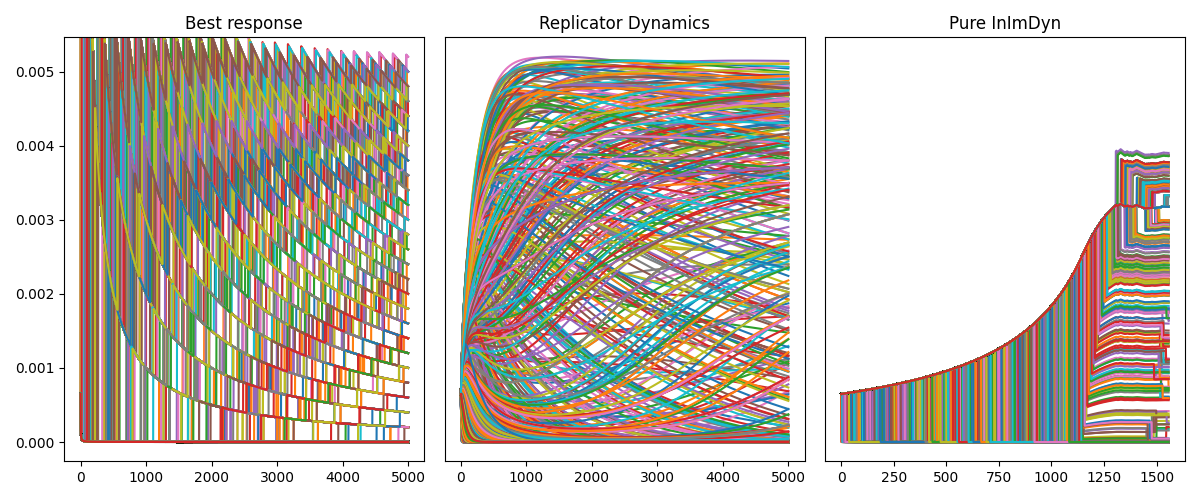
\includegraphics[width=0.8\textwidth]{../figures/trajectories/102061.png}
        \caption{Trajectories of the mixed strategy entries on the first segment of two images from the BSDS300 dataset}
        \label{fig:trajectories}
    \end{figure}
    The figure above shows that with the same number of iterations, the \textit{Infection and immunization dynamics} reaches a stable state faster than the two other strategies.
\end{frame}

\begin{frame}
    \frametitle{Semantic segmentation with deep self-supervised DINO features}
    \begin{figure}
        \centering
        \begin{subfigure}[b]{0.16\textwidth}
            \centering
            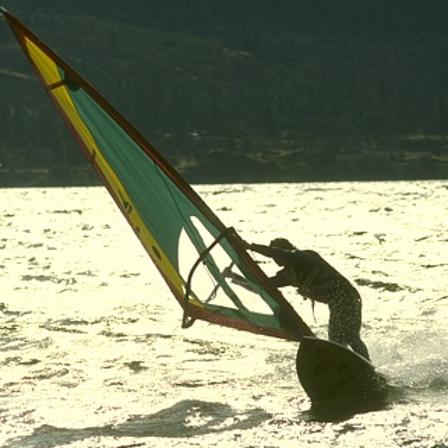
\includegraphics[width=\textwidth]{../figures/dino/tile_2/62096.jpg}
            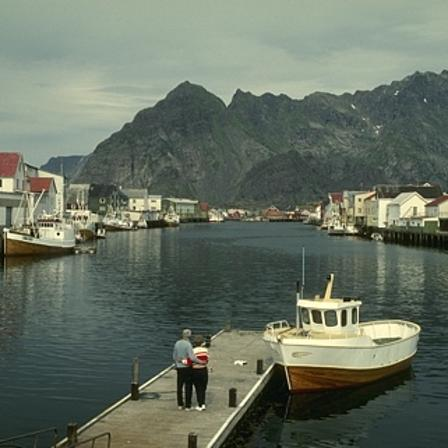
\includegraphics[width=\textwidth]{../figures/dino/tile_2/219090.jpg}
            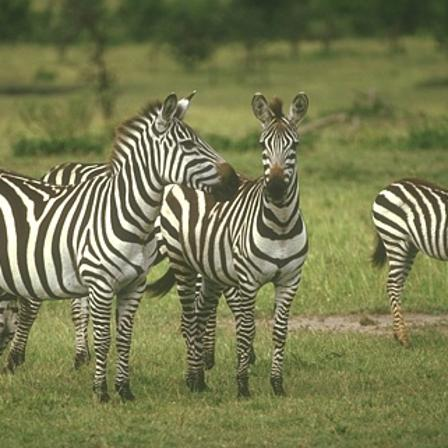
\includegraphics[width=\textwidth]{../figures/dino/tile_2/253027.jpg}
            \caption{Original}
        \end{subfigure}
        \hfill
        \begin{subfigure}[b]{0.16\textwidth}
            \centering
            
\includegraphics[width=\textwidth]{../figures/dino/tile_2/62096_seg.png}
            
\includegraphics[width=\textwidth]{../figures/dino/tile_2/219090_seg.png}
            
\includegraphics[width=\textwidth]{../figures/dino/tile_2/253027_seg.png}
            \caption{Clusters}
        \end{subfigure}
        \hfill
        \begin{subfigure}[b]{0.16\textwidth}
            \centering
            
\includegraphics[width=\textwidth]{../figures/dino/tile_2/62096_avg.png}
            
\includegraphics[width=\textwidth]{../figures/dino/tile_2/219090_avg.png}
            
\includegraphics[width=\textwidth]{../figures/dino/tile_2/253027_avg.png}
            \caption{Average colors}
        \end{subfigure}
           \caption{Segmentations obtained with DINO features on $4$ tiles of $28\times 28$.}
           \label{fig:results-dino-tile2}
    \end{figure}
\end{frame}

\begin{frame}
    \frametitle{Implementation}
    We provide all the sources to reproduce our results on the BSDS300\cite{bsds300} dataset as a Jupyter Notebook. Feel free to consult it at:
    \begin{center}
        \url{https://github.com/clementjambon/evolutionary-segmentation}
    \end{center}
\end{frame}

\begin{frame}[shrink=30]
\bibliographystyle{plain}
\bibliography{../biblio.bib}  
\end{frame}
  

\end{document}